We designed and built an open source web application, OPQHub, that provides local and global displays of PQ data. Our service collects, aggregates, and analyzes PQ data from a set of distributed PQ meters (figure \ref{fig:opqhub}).

\begin{figure*}
  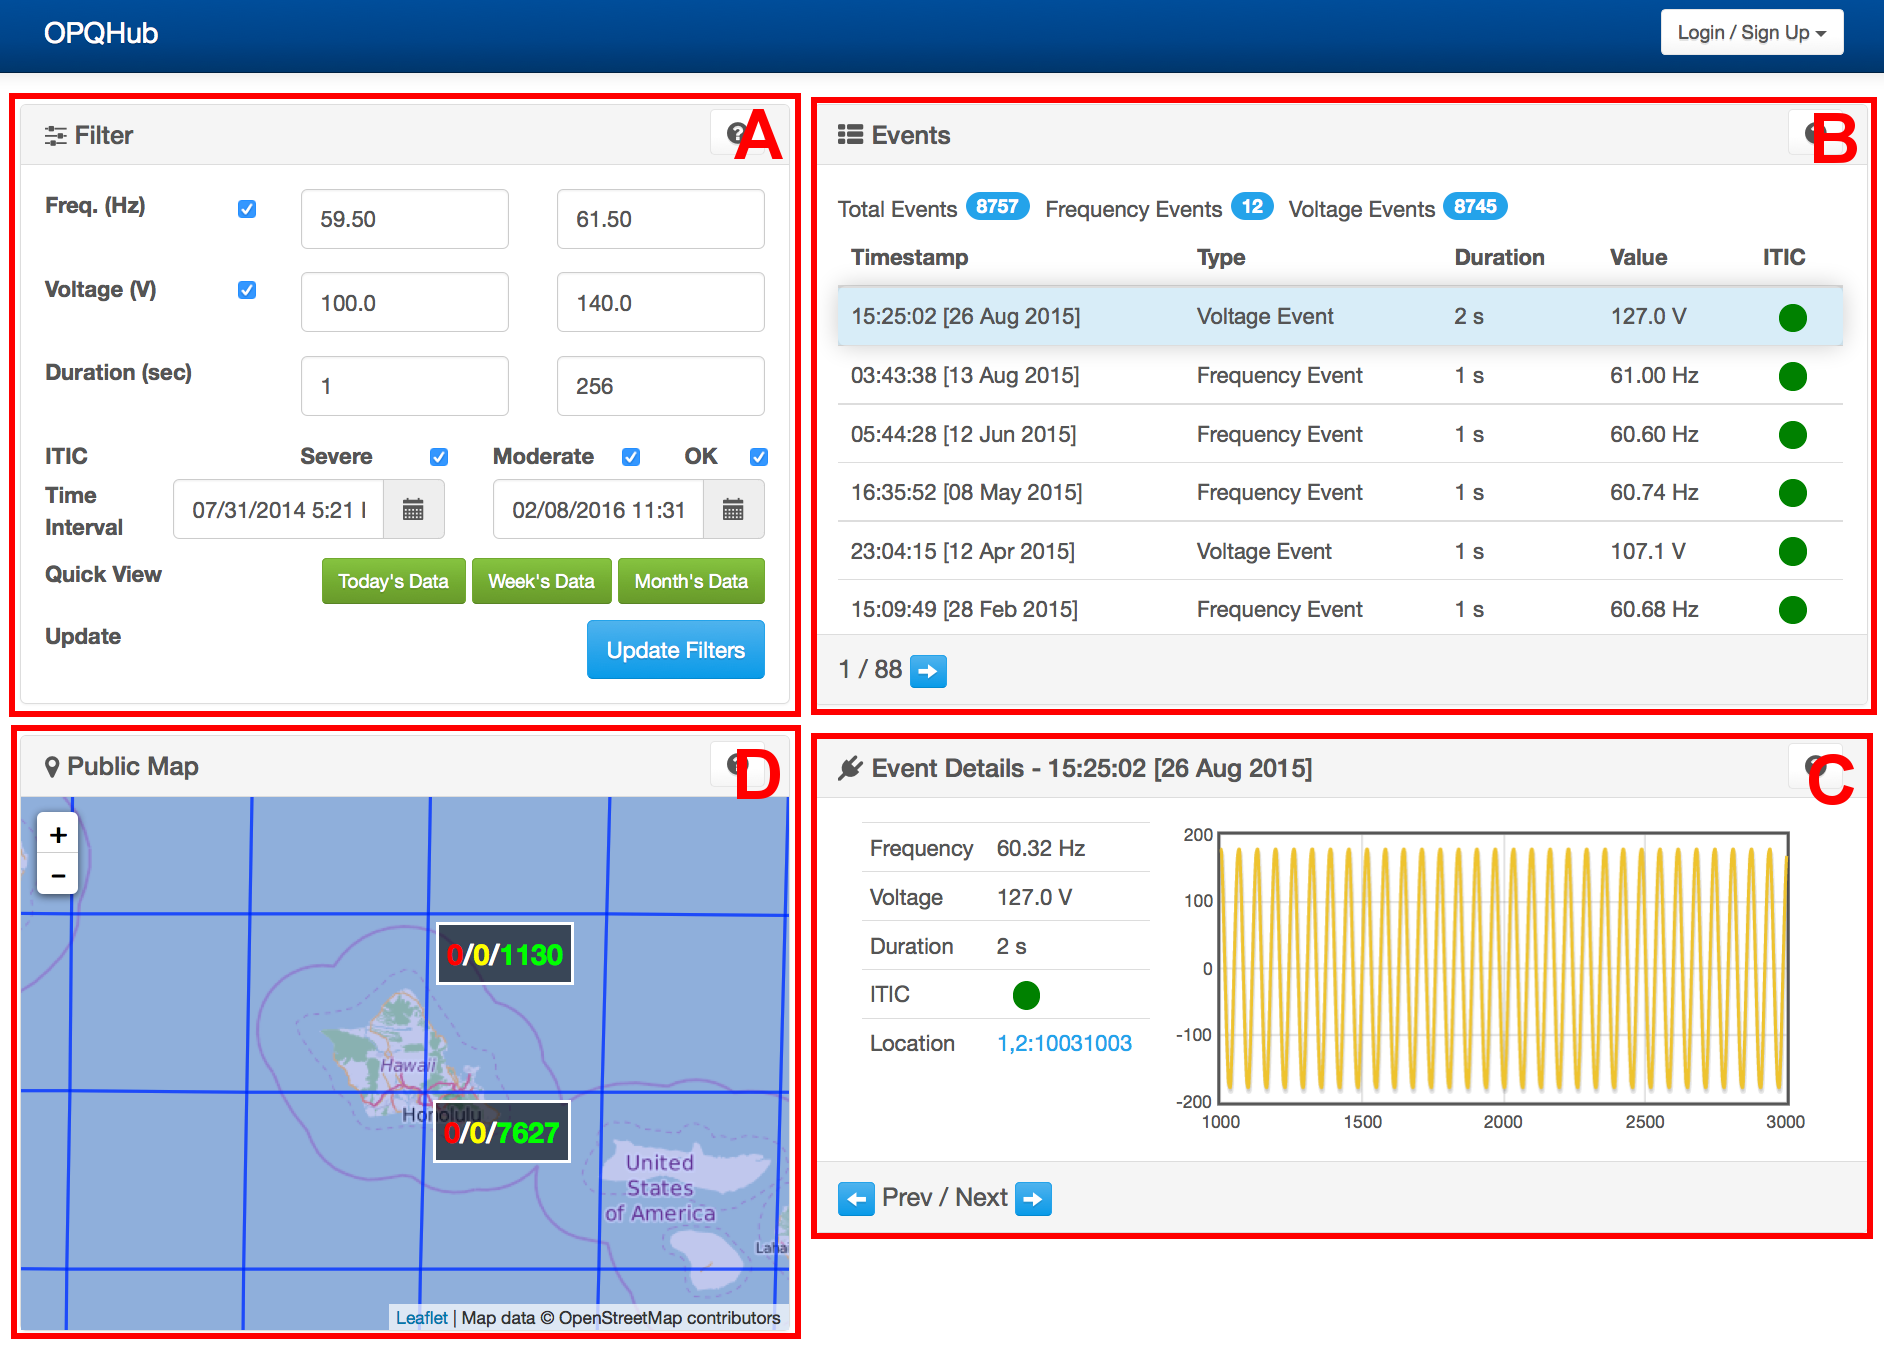
\includegraphics[width=\textwidth,height=13cm]{img/opqhub.png}
  \caption{OPQHub Distributed PQ Event and Information Reporting Interface. A) PQ events can be queried and filtered over complex criteria. B) List of PQ events that match filtered criteria. C) Details of a single PQ event. D) Dynamic map visualization of PQ events and query filter.}
  \label{fig:opqhub}
\end{figure*}

\subsection{Querying}
We provide facilities to query PQ events reported to our system by filtering on the following items: date, duration, min voltage, max voltage, min frequency, max frequency, severity as defined by the ITIC curve\cite{m:ITIC}, and location. Location queries are performed by using a bounding box given by the currently viewable area in a dynamic map interface.

A successful query returns a list of PQ events that meet the provided criteria. These events contain details about where and when the PQ event took place as well as raw waveform data that can be displayed using our interface.

\subsection{Quadtree Based Event Reporting}
A useful tool when working with any geographically distributed data set is a dynamic map to visualize events and other related information. We came across several issues when designing a map interface to display PQ events and information.

First, how can we maintain our users' privacy if a map displays the exact location of PQ events? We initially tried providing a randomization mechanism that would smudge the exact location randomly by some amount, but this didn't solve our second problem. Displaying multiple events generated by sensors that are close in time and location quickly clutter the map and reduced the amount of information available.

Building upon the open source map library Leaflet, we created a quadtree based grid visualization for displaying PQ events and related information that solves the issues related to users' privacy and multiple events being generated in the same location.

Instead of displaying PQ events as individual icons, the system utilizes GeoJson to display an aggregate count of events that are represented by the bounding box that forms a grid square. As the user zooms out, grids are combined together and the counts are combined into a more course grid layout. As the user zooms in, the grid squares are subdivided and the counts become more spread out and granular.

\subsubsection{Quadtree Based Grid Generation}
The top layer of our tree consists of a grid of squares where each square is 256 kilometers x 256 kilometers wide. Each top level grid square is then recursively subdivided into four squares of equals width. 

Our map was optimized to work with the state of Hawaii. Different parameters need to be chosen for using this map for other areas. For example, a larger state may require a courser or finer set of top level grid squares.

To generate an evenly spaced grid, we identified the NW and SE latitude and longitude points of the bounding box (BB) that contains the area of interest our grid should cover. The BB we chose for Hawaii is outlined in table \ref{tab:bb_hawaii}.

\begin{table}[htbp]
	\caption{Hawaii Grid Square Bounding Box}
	\label{tab:bb_hawaii}
	\begin{center}
		\begin{tabular}{|l|r|r|r|}
			\hline
			\textbf{BB Point} & \textbf{ Location} & \textbf{Latitude} & \textbf{Longitude}\\
			\hline
			North West & NW of Niihau & 22.534353 & -161.004639\\
			\hline
			South East & SE of Big Island & 16.719592 & -151.853027\\
			\hline
		\end{tabular} 
	\end{center}
\end{table}

We can calculate the latitude ($\phi$) and longitude ($\lambda$) of a point $(\phi_2, \lambda_2)$, given a starting point $(
\phi_1, \lambda_1)$, bearing ($\Theta$), distance ($d$), and angular distance ($AD=\frac{d}{radius\ of\ earth}$) with the following formula which uses the distance over a great arc circle as an approximation for the shape of the earth \cite{w:calc_lat_lng}.

$\phi_2 = asin(sin(\phi_1 * cos(AD) + cos(\phi_1) + sin(AD) * cos(\Theta))$

$\lambda_2 = \lambda_1 + atan2(sin(\Theta) * sin(AD) * cos(\phi_1), cos(AD) - sin(\phi_1) * sin(\phi_2))$

With the above formula, we start with the NW point of the BB, and generate all points due South of the starting point within the BB with a given distance interval. This process generates the first point for each of the row in our point matrix. Then for each starting point, we generate all points due East within the BB. The result of this process is a matrix of evenly spaced points which can then be used to create polygons of evenly spaced grid squares.

\subsubsection{Quadtree Based Geo-Hashing}
Our quadtree approach allows us to easily bin locations within a grid square at a given depth in the tree. Because of it's rigid structure, it's easy to use this data structure to perform geo-hashing of locations. The scheme we chose is as follows.

In order to associate OPQ hardware devices with locations on the grid, we developed a naming scheme that stores the parent information of each grid in the name itself. Grids at the coarsest grid scale (256 kilometers) are simply named by their row ($r$) and column ($c$) using the format $r,c:$. We show an example of how the coarsest grid squares would be named in figure \ref{fig:coarsest_grid_ids}.

\begin{figure}[htbp]
	\centering
	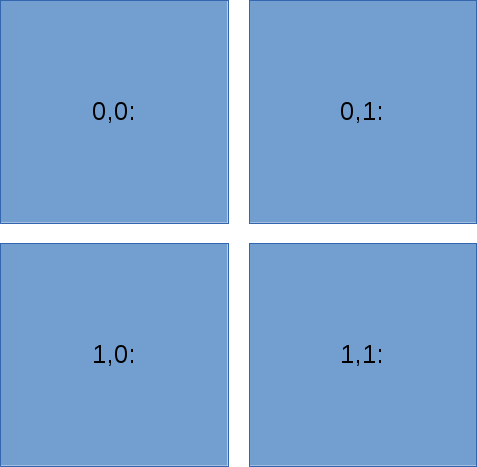
\includegraphics[width=0.6\columnwidth]{img/grid-sq.png}
	\caption{Naming Convention for Coarsest Grid Layer.}
	\label{fig:coarsest_grid_ids}
\end{figure}

For each level that the grid becomes more fine, each square recursively divides into four squares. We can name each of these child squares by its location in the parent square. For each finer level, we simply append this location id onto its parent's id.

\begin{table}[htbp]
	\caption{Naming of Child Grid Squares}
	\label{tab:grid_first_child}
	\begin{center}
		\begin{tabular}{|l|r|}
			\hline
			\textbf{Position in Parent} & \textbf{ID}\\
			\hline
			Top Left & 0\\
			\hline
			Top Right & 1\\
			\hline
			Bottom Right & 2\\
			\hline
			Bottom Left & 3\\
			\hline
		\end{tabular} 
	\end{center}
\end{table}

Figure \ref{fig:coarsest_grid_ids} shows the ids of the first level of children under the parent grid square.

%\begin{figure}[htbp]
%	\centering
%	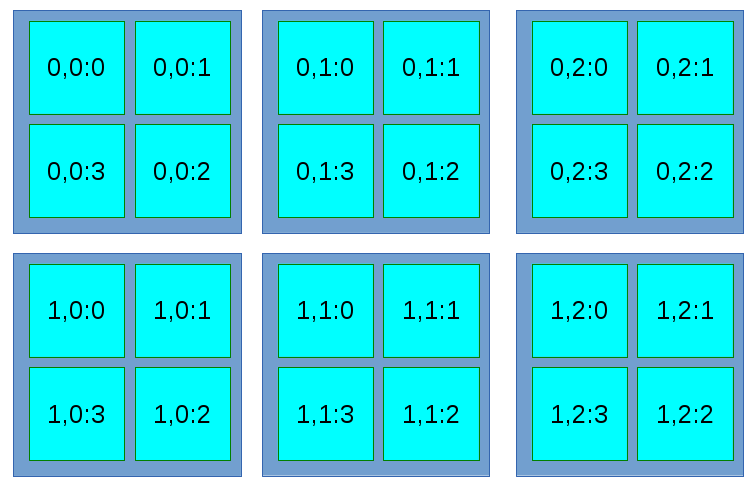
\includegraphics[width=0.8\columnwidth]{img/grid-sq-1.png}
%	\caption{Naming Convention for First Children.}
%	\label{fig:first_children}
%\end{figure}

We can then recursively use the same naming scheme for each level of children in the grid. For example, a grid id of ``0,0:13" represents the following information. At the coarsest level, the location ``0,0:" represents the top left 256x256 kilometer grid square. The following ``1" represents that the 128x128 kilometer child of the coarsest level is located at the top right of its parent square. The following ``3" represents that the grandchild of the coarsest square is in the bottom left of the child's square. To illustrate the concept of recursive ids, please refer to \ref{fig:second_children}.

\begin{figure}[htbp]
	\centering
	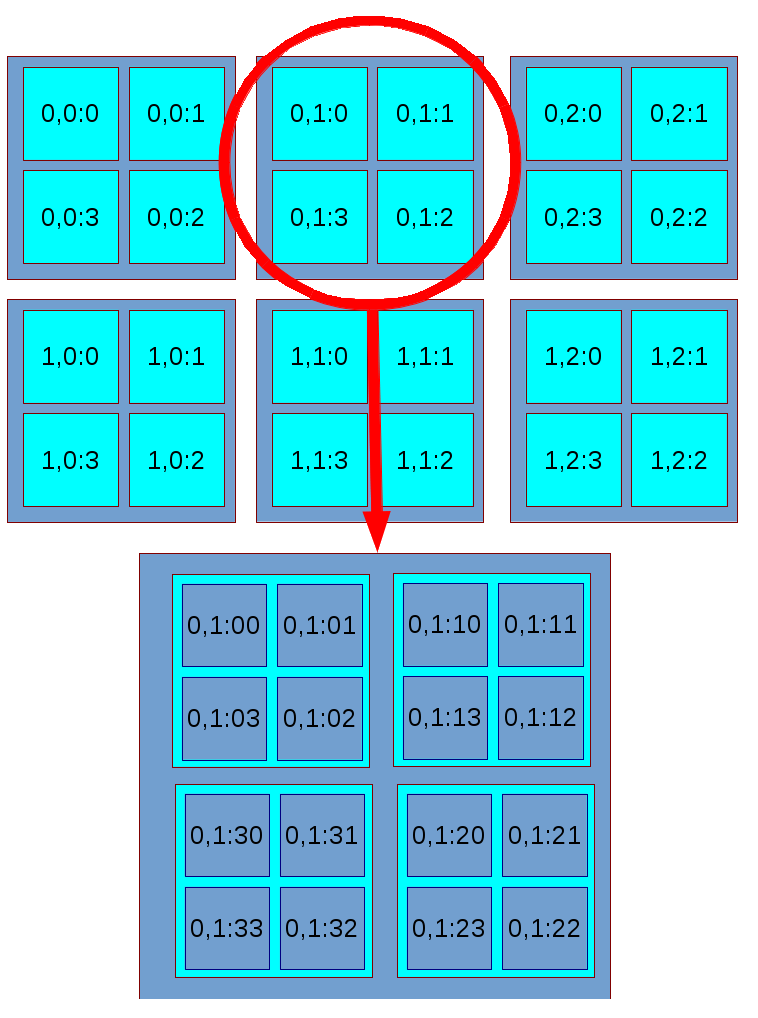
\includegraphics[width=0.8\columnwidth]{img/grid-sq-2.png}
	\caption{Recursive Naming of Children.}
	\label{fig:second_children}
\end{figure}

\begin{figure*}[htbp]
	\centering
	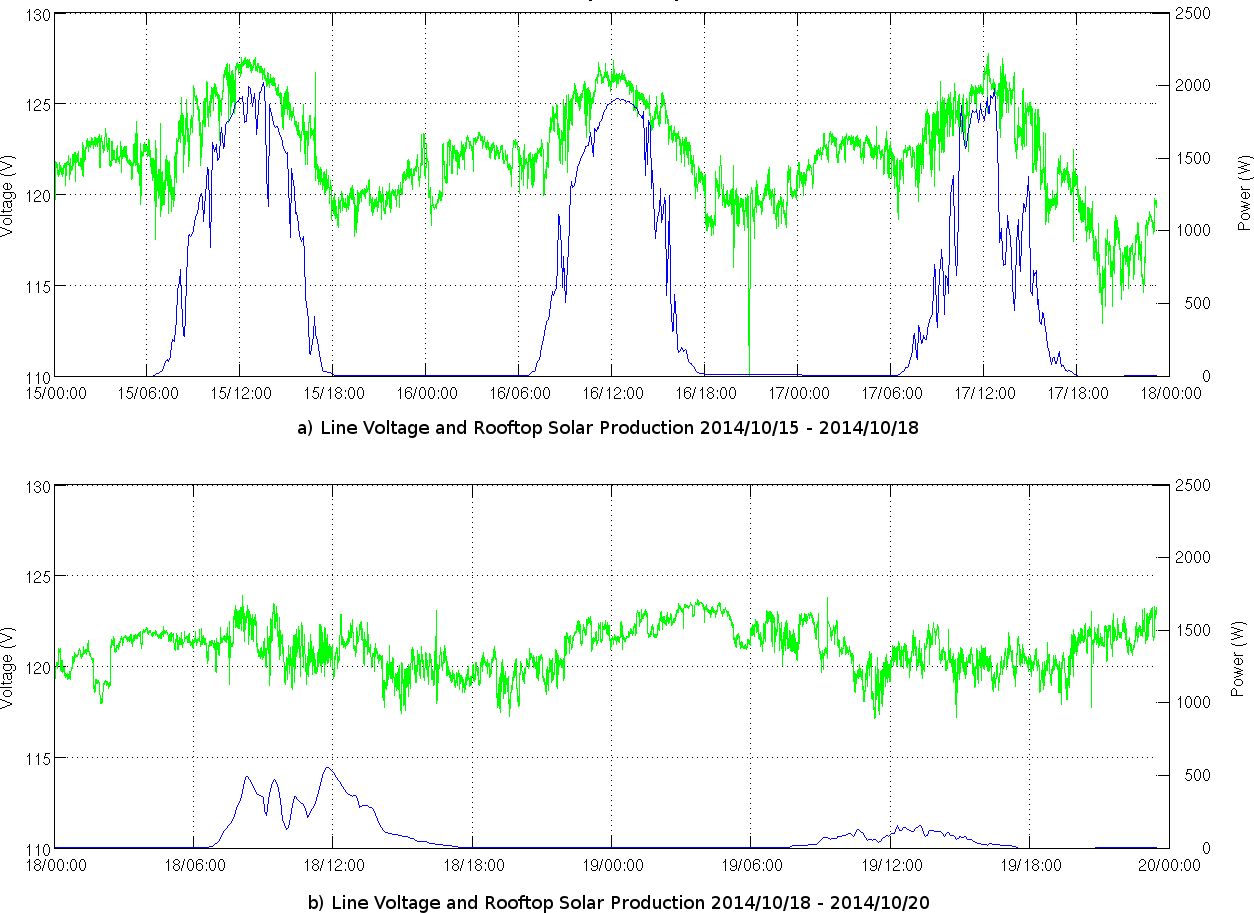
\includegraphics[width=0.8\textwidth]{img/weatherTrends.png}
	\caption{Top graph shows the residential line to neutral voltage and rooftop solar production during a sunny day on the Island of Oahu. Bottom graph shows the voltage and solar production during Hurricane Ana.}
	\label{fig:opqbox1}
\end{figure*}

\subsubsection{Dynamic Sizing of Grid}
Grid scale is defined as the length of each square polygon in the grid. That is, a grid scale of 256 kilometers contains grid squares which each are 256 kilometers by 256 kilometers. The coarsest grid scale that we support is 256 kilometers and the finest grid scale is $\frac{1}{8}$ kilometer.

We designed our grid-map library so that when the map is zoomed out, it displays the coarsest grid of 256 kilometers. As the map is zoomed in, each grid square is recursively divided into four smaller squares, each with a grid-scale that is exactly one-half of its parent's. This process continues until the map is at max zoom and each grid square represents $\frac{1}{8}$ of a kilometer.

The location of any grid is invariant to both zoom and pan as long as the NE BB starting point is not changed. This makes it easy to associate ids with individual grid squares so that devices can then be associated with individual grid squares.

\subsubsection{Privacy Gained From Quadtree Approach}
If a user decides to include their location, they are able to select a grid square at a depth that they are comfortable and that describes their location. If a user is not as concerned about their privacy, they can select a grid square that might enclose their house. If a user is more privacy conscious, they might select a grid square that contains their block, their neighborhood, or an entire island. We empower our users to select a coarseness of location which suits their privacy needs.





